% ------------------------------------------------------------------------------
% TYPO3 CMS 7.2 - What's New - Chapter "Introduction" (English Version)
%
% @author	Michael Schams <schams.net>
% @license	Creative Commons BY-NC-SA 3.0
% @link		http://typo3.org/download/release-notes/whats-new/
% @language	English
% ------------------------------------------------------------------------------
% LTXE-CHAPTER-UID:		16517900-07a67f43-fe9f3e35-7e924788
% LTXE-CHAPTER-NAME:	Introduction
% ------------------------------------------------------------------------------

\section{Inleiding}
\begin{frame}[fragile]
	\frametitle{Inleiding}

	\begin{center}\huge{Inleiding}\end{center}
	\begin{center}\huge{\color{typo3darkgrey}\textbf{De feiten}}\end{center}

\end{frame}

% ------------------------------------------------------------------------------
% LTXE-SLIDE-START
% LTXE-SLIDE-UID:		349ac766-32c0ba00-d7251be6-87970e29
% LTXE-SLIDE-ORIGIN:	6d5e9f3e-f9d9677e-43d7d497-e80ba9ef English
% LTXE-SLIDE-TITLE:		TYPO3 CMS 7.2 - The Facts
% ------------------------------------------------------------------------------
\begin{frame}[fragile]
	\frametitle{Inleiding}
	\framesubtitle{TYPO3 CMS 7.2 - De feiten}

	\begin{itemize}
		\item Publicatiedatum: 28 april 2015
		\item Publicatietype: "Sprint Release"
		\item Visie: Omarm, Innoveer, Verspreid
		\item Primaire focus: Frontend
	\end{itemize}

	\begin{figure}
		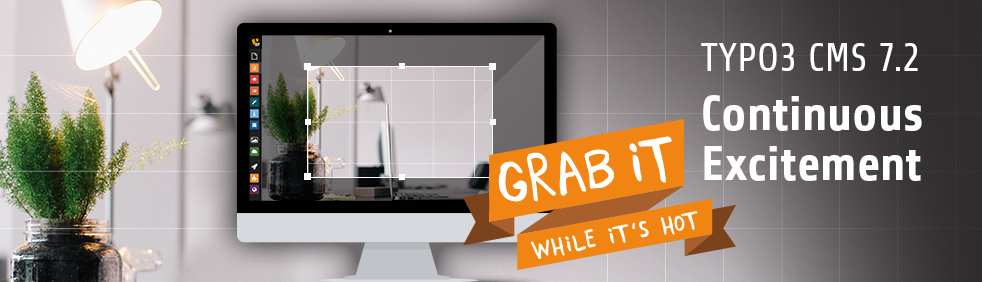
\includegraphics[width=0.95\linewidth]{Introduction/typo3cms72-teaser.png}
	\end{figure}

\end{frame}

% ------------------------------------------------------------------------------
% LTXE-SLIDE-START
% LTXE-SLIDE-UID:		d5f6cce1-c9aa0c53-148efb47-f4afd1c0
% LTXE-SLIDE-ORIGIN:	759c3860-d5061f6e-2bb0009f-6ea130c8 English
% LTXE-SLIDE-TITLE:		System Requirements
% ------------------------------------------------------------------------------
\begin{frame}[fragile]
	\frametitle{Inleiding}
	\framesubtitle{Systeemvereisten}

	\begin{itemize}
		\item PHP*:\tabto{2.2cm}v5.5.0 - v5.6.x
		\item MySQL:\tabto{2.2cm}v5.5.x - v5.6.x (no strict mode)
		\item Schijfruimte:\tabto{2.2cm}min 200 MB
		\item PHP-instellingen:

			\begin{itemize}
				\item memory\_limit >= 128M
				\item max\_execution\_time >= 240s
				\item compilation option \texttt{--disable-ipv6} \underline{niet} gebruiken
			\end{itemize}

		\item Backend vereist IE >= 9 of een andere moderne browsers

	\end{itemize}

	\vspace{1cm}
	*) Meer details: \href{http://typo3.org/news/article/php-minimum-requirements-for-typo3-cms-7/}{PHP Minimum Requirements for TYPO3 CMS 7}

\end{frame}

% ------------------------------------------------------------------------------
% LTXE-SLIDE-START
% LTXE-SLIDE-UID:		532e1f03-d16ad3b3-2078065b-bf20acfc
% LTXE-SLIDE-ORIGIN:	70c77c41-e2b83d82-2f182996-98061070 English
% LTXE-SLIDE-TITLE:		Development And Release Timeline
% ------------------------------------------------------------------------------
\begin{frame}[fragile]
	\frametitle{Inleiding}
	\framesubtitle{Ontwikkelings- en publicatietijdlijn}

	\begin{figure}
		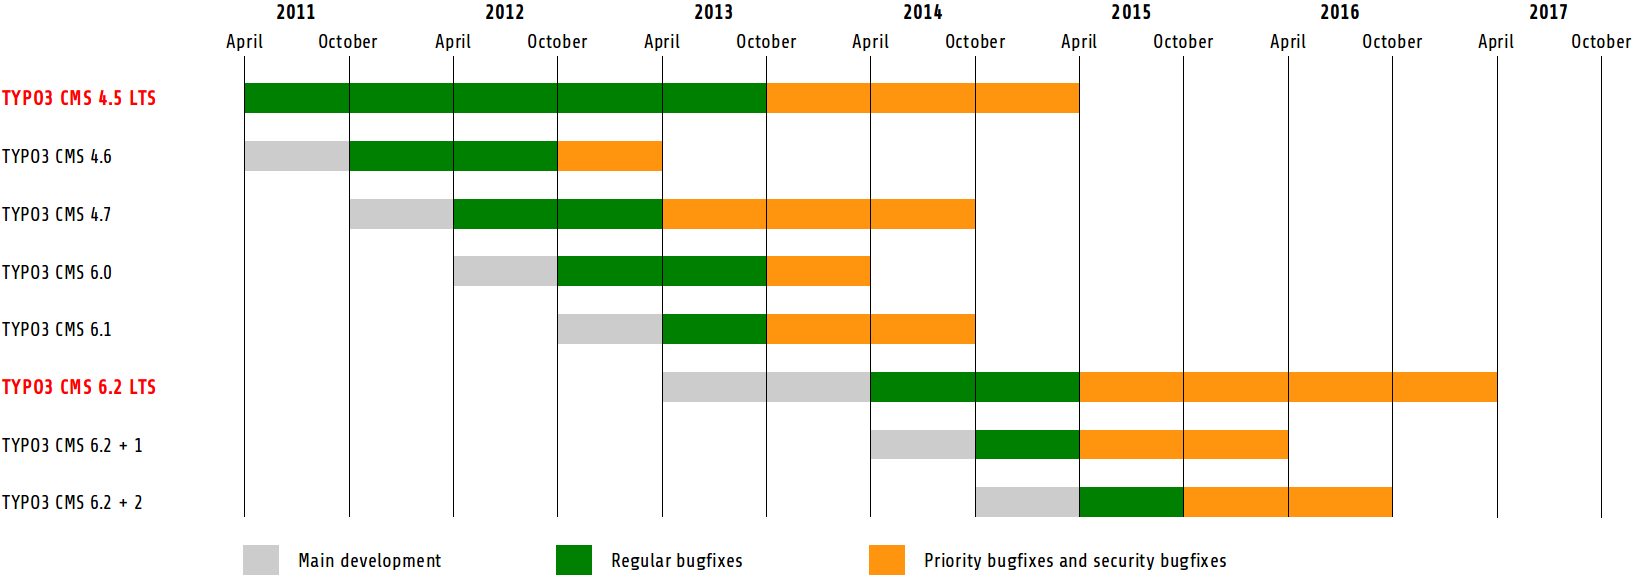
\includegraphics[width=0.90\linewidth]{Introduction/ReleaseAgenda.png}
	\end{figure}

\end{frame}

% ------------------------------------------------------------------------------
% LTXE-SLIDE-START
% LTXE-SLIDE-UID:		0e405de9-be73c1c7-73b6ff73-b9e537e6
% LTXE-SLIDE-ORIGIN:	b55d3fe9-76807061-d97f3fee-7db1f190 English
% LTXE-SLIDE-TITLE:		TYPO3 CMS Roadmap
% ------------------------------------------------------------------------------
\begin{frame}[fragile]
	\frametitle{Inleiding}
	\framesubtitle{TYPO3 CMS Roadmap}

	Geschatte publicatiedatum en primaire focus:

	\begin{itemize}
		\item v7.0 \tabto{1.0cm}02/dec/2014\tabto{3.4cm}Backend makeover deel 1
		\item v7.1 \tabto{1.0cm}24/feb/2015\tabto{3.4cm}Core opschonen en stroomlijnen

		\item
			\begingroup
				\color{typo3orange}
					v7.2 \tabto{1.0cm}28/apr/2015\tabto{3.4cm}Frontend
			\endgroup

		\item v7.3 \tabto{1.0cm}09/jun/2015\tabto{3.4cm}Package Ecosysteem, Composer\newline
			\tabto{3.4cm}en Extensie-afhandeling
		\item v7.4 \tabto{1.0cm}04/aug/2015\tabto{3.4cm}Backend makeover deel 2
		\item v7.5 \tabto{1.0cm}29/sep/2015\tabto{3.4cm}\textit{(nog vast te stellen...)}
		\item v7.6 \tabto{1.0cm}xx/xxx/2015\tabto{3.4cm}\textbf{TYPO3 CMS 7 LTS} (Long Term Release)
	\end{itemize}

	\smaller
		\url{https://typo3.org/typo3-cms/roadmap/}\newline
		\url{http://typo3.org/news/article/embrace-and-innovate-typo3-cms-7/}
	\normalsize

\end{frame}

% ------------------------------------------------------------------------------
% LTXE-SLIDE-START
% LTXE-SLIDE-UID:		91327b47-490e22cc-8434b9ea-c8406daa
% LTXE-SLIDE-ORIGIN:	b0c28f26-c3ca2e99-195954a8-ed76f9d4 English
% LTXE-SLIDE-TITLE:		Installation
% ------------------------------------------------------------------------------
\begin{frame}[fragile]
	\frametitle{Inleiding}
	\framesubtitle{Installatie}

	\begin{itemize}
		\item Officiële installatieprocedure op Linux/Mac OS X\newline
			(DocumentRoot bijvoorbeeld \texttt{/var/www/site/htdocs}):
		\begin{lstlisting}
			$ cd /var/www/site
			$ wget --content-disposition get.typo3.org/7.2
			$ tar xzf typo3_src-7.2.0.tar.gz
			$ cd htdocs
			$ ln -s ../typo3_src-7.2.0 typo3_src
			$ ln -s typo3_src/index.php
			$ ln -s typo3_src/typo3
			$ touch FIRST_INSTALL
		\end{lstlisting}

		\item Symbolische koppelingen op Microsoft Windows:

			\begin{itemize}
				\item Gebruik \texttt{junction} met Windows XP/2000
				\item Gebruik \texttt{mlink} met Windows Vista en Windows 7
			\end{itemize}

	\end{itemize}
\end{frame}

% ------------------------------------------------------------------------------
% LTXE-SLIDE-START
% LTXE-SLIDE-UID:		9372da37-6d52062b-94a6fbca-6d599d86
% LTXE-SLIDE-ORIGIN:	48136734-ae508d23-bce5811d-667f8908 English
% LTXE-SLIDE-TITLE:		Upgrade to TYPO3 CMS 7
% ------------------------------------------------------------------------------
\begin{frame}[fragile]
	\frametitle{Inleiding}
	\framesubtitle{Upgrade naar TYPO3 CMS 7.x}

	\begin{itemize}
		\item Upgrade alleen mogelijk van TYPO3 CMS 6.2 LTS
		\item TYPO3 CMS < 6.2 moet eerst naar TYPO3 CMS 6.2 LTS gezet worden
	\end{itemize}

	\begin{itemize}

		\item Upgrade-instructies:\newline
			\smaller\url{http://wiki.typo3.org/Upgrade#Upgrading_to_7.2}\normalsize
		\item Officiële TYPO3 handleiding "TYPO3 Installation and Upgrading":
			\smaller\url{http://docs.typo3.org/typo3cms/InstallationGuide}\normalsize
		\item Algemene aanpak:
			\begin{itemize}
				\item Controleer minimale systeemvereisten (PHP, MySQL, etc.)
				\item Check \textbf{deprecation\_*.log} in oude TYPO3 installatie
				\item Werk alle extensies bij naar nieuwste versie
				\item Zet nieuwe bronbestanden neer en start Install Tool \textrightarrow Upgrade Wizard
				\item Check startmodule voor backend gebruikers (optioneel)
			\end{itemize}
	\end{itemize}

\end{frame}

% ------------------------------------------------------------------------------
